\clearpage
\part{Assignment 5: Measuring the Accuracy and Precision of a KUKA youBot Arm}

\section{Experimental Setup}
\begin{itemize}
    \item \textbf{Hardware:}
    \begin{itemize}
        \item A KUKA youBot arm placed on a table in the C069 lab.
        \item A computer used for controlling the arm.
        \item Objects with three different sizes (small, medium, and large) used for picking and placing.
        \item Visual markers attached on the top of the objects.
        \item An external tracking system (OptiTrack Motion Tracking System) placed above the robot’s workspace and connected to an additional PC.
        \item A fixed template on the table to ensure constant initial object position.
    \end{itemize}
    \item \textbf{Software:}
    \begin{itemize}
        \item KUKA youBot drivers for controlling the arm.
        \item Additional control script with pre-saved pick and place poses.
        \item Rosbag recorder for recording the end-effector path.
        \item Motive software for visualizing, recording, and exporting tracking data as CSV.
    \end{itemize}
    
    \item \textbf{Issues Faced:} 
    \begin{itemize}
        \item The arm was failing randomly, the driver would stop responding and the arm would not move at all. We had to restart the terminals.
        \item The OptiTrack system was not able to differentiate between the medium and large object.
        \item The export settings on the Motive software was not set according to the expected frame.
    \end{itemize}
\end{itemize}



\section{Experiment Execution}
\begin{itemize}
    \item \textbf{Procedure:} 
    \begin{itemize}
        \item Started roscore, youbot driver, moveit move group, and youBot placing experiment in separate terminals.
        \item Used the control script to perform pick and place for each object(small, medium and large) and pose combination(straight, left, and right).
        \item Recorded poses using OptiTrack Motive in live mode, naming takes, starting and stopping recordings, and exporting to CSV.
        \item Recorded internal end-effector positions via ROS bagfiles, later converted to CSV using the provided script.
    \end{itemize}
    \item \textbf{Trials:} 25 trials per object-place combination (3 sizes × 3 positions = 9 combinations), totaling 225 trials.
    \item \textbf{Poses Captured:} Final object poses from OptiTrack (external) and end-effector poses from ROS (internal) for each trial.
\end{itemize}



\section{Observations During Execution}
\begin{itemize}
    \item The arm performed movements reliably, but larger object used to wobble a lot before settling down to stable position.
    \item Possible Error Sources:
    \begin{itemize}
        \item Occlusion of OptiTrack markers by the arm during motion.
        \item Joint encoder inaccuracies in the youBot arm, leading to biased internal measurements.
        \item Environmental factors like table vibrations or air currents affecting light objects, but mostly ensured table and external factors were mostly stable during the experiment.
    \end{itemize}
\end{itemize}



\section{Pose Filtering Procedure}
To preprocess the data and remove outliers, we applied the Interquartile Range (IQR) method to the x and y coordinates of the end-effector poses obtained from the youBot's internal encoders. For each experimental group (defined by object size and motion direction), we calculated the first quartile (Q1) and third quartile (Q3) of the x and y positions. Outliers were identified as points falling below Q1 - 1.5*IQR or above Q3 + 1.5*IQR in either coordinate. These outliers were removed from the dataset.

Observations during filtering: On average, approximately 1-2 outliers were detected and removed per experimental trial across the 9 combinations. Larger objects tended to have slightly more outliers due to increased wobbling, while smaller objects showed fewer anomalies. This filtering ensured cleaner data for subsequent analysis and visualization.

% \newpage

% \section{Preprocessed Data}
% The preprocessed data was saved as a CSV file named \texttt{preprocessed\_data.csv} with the following structure:
% \begin{itemize}
%     \item Columns: mass (small/medium/large), position (left/right/straight), trial (1-25), type (external/internal), x, y, theta
% \end{itemize}

% \paragraph{Sample Data:}
% \begin{lstlisting}
% mass,position,trial,type,x,y,theta
% small,left,1,external,29.8,-35.3,0.0
% small,left,1,internal,29.8,-35.3,0.0
% small,left,2,external,29.8,-35.3,0.0
% ... (full data in preprocessed_data.csv)
% \end{lstlisting}

\section{Data Merging}
The individual CSV was merged with data from classmates by concatenating all preprocessed CSVs into a single DataFrame. This combined dataset was used for visualizations and analysis. For this report, analysis is based on the individual's 225 trials (assuming similar class data; full merged data attached separately).



\section{Visualization of Poses}
Visualizations were created using scatter plots to illustrate the distribution of final object and end-effector poses for each object size, combining all motion directions (straight, left, right) in a single plot. Directions are differentiated by colors: blue for straight, green for left, red for right. A clear distinction is made between externally tracked poses (OptiTrack, X markers) and internally sensed positions (youBot encoders, shaped markers). Arrows indicate orientation.

\begin{figure}[H]
    \centering
    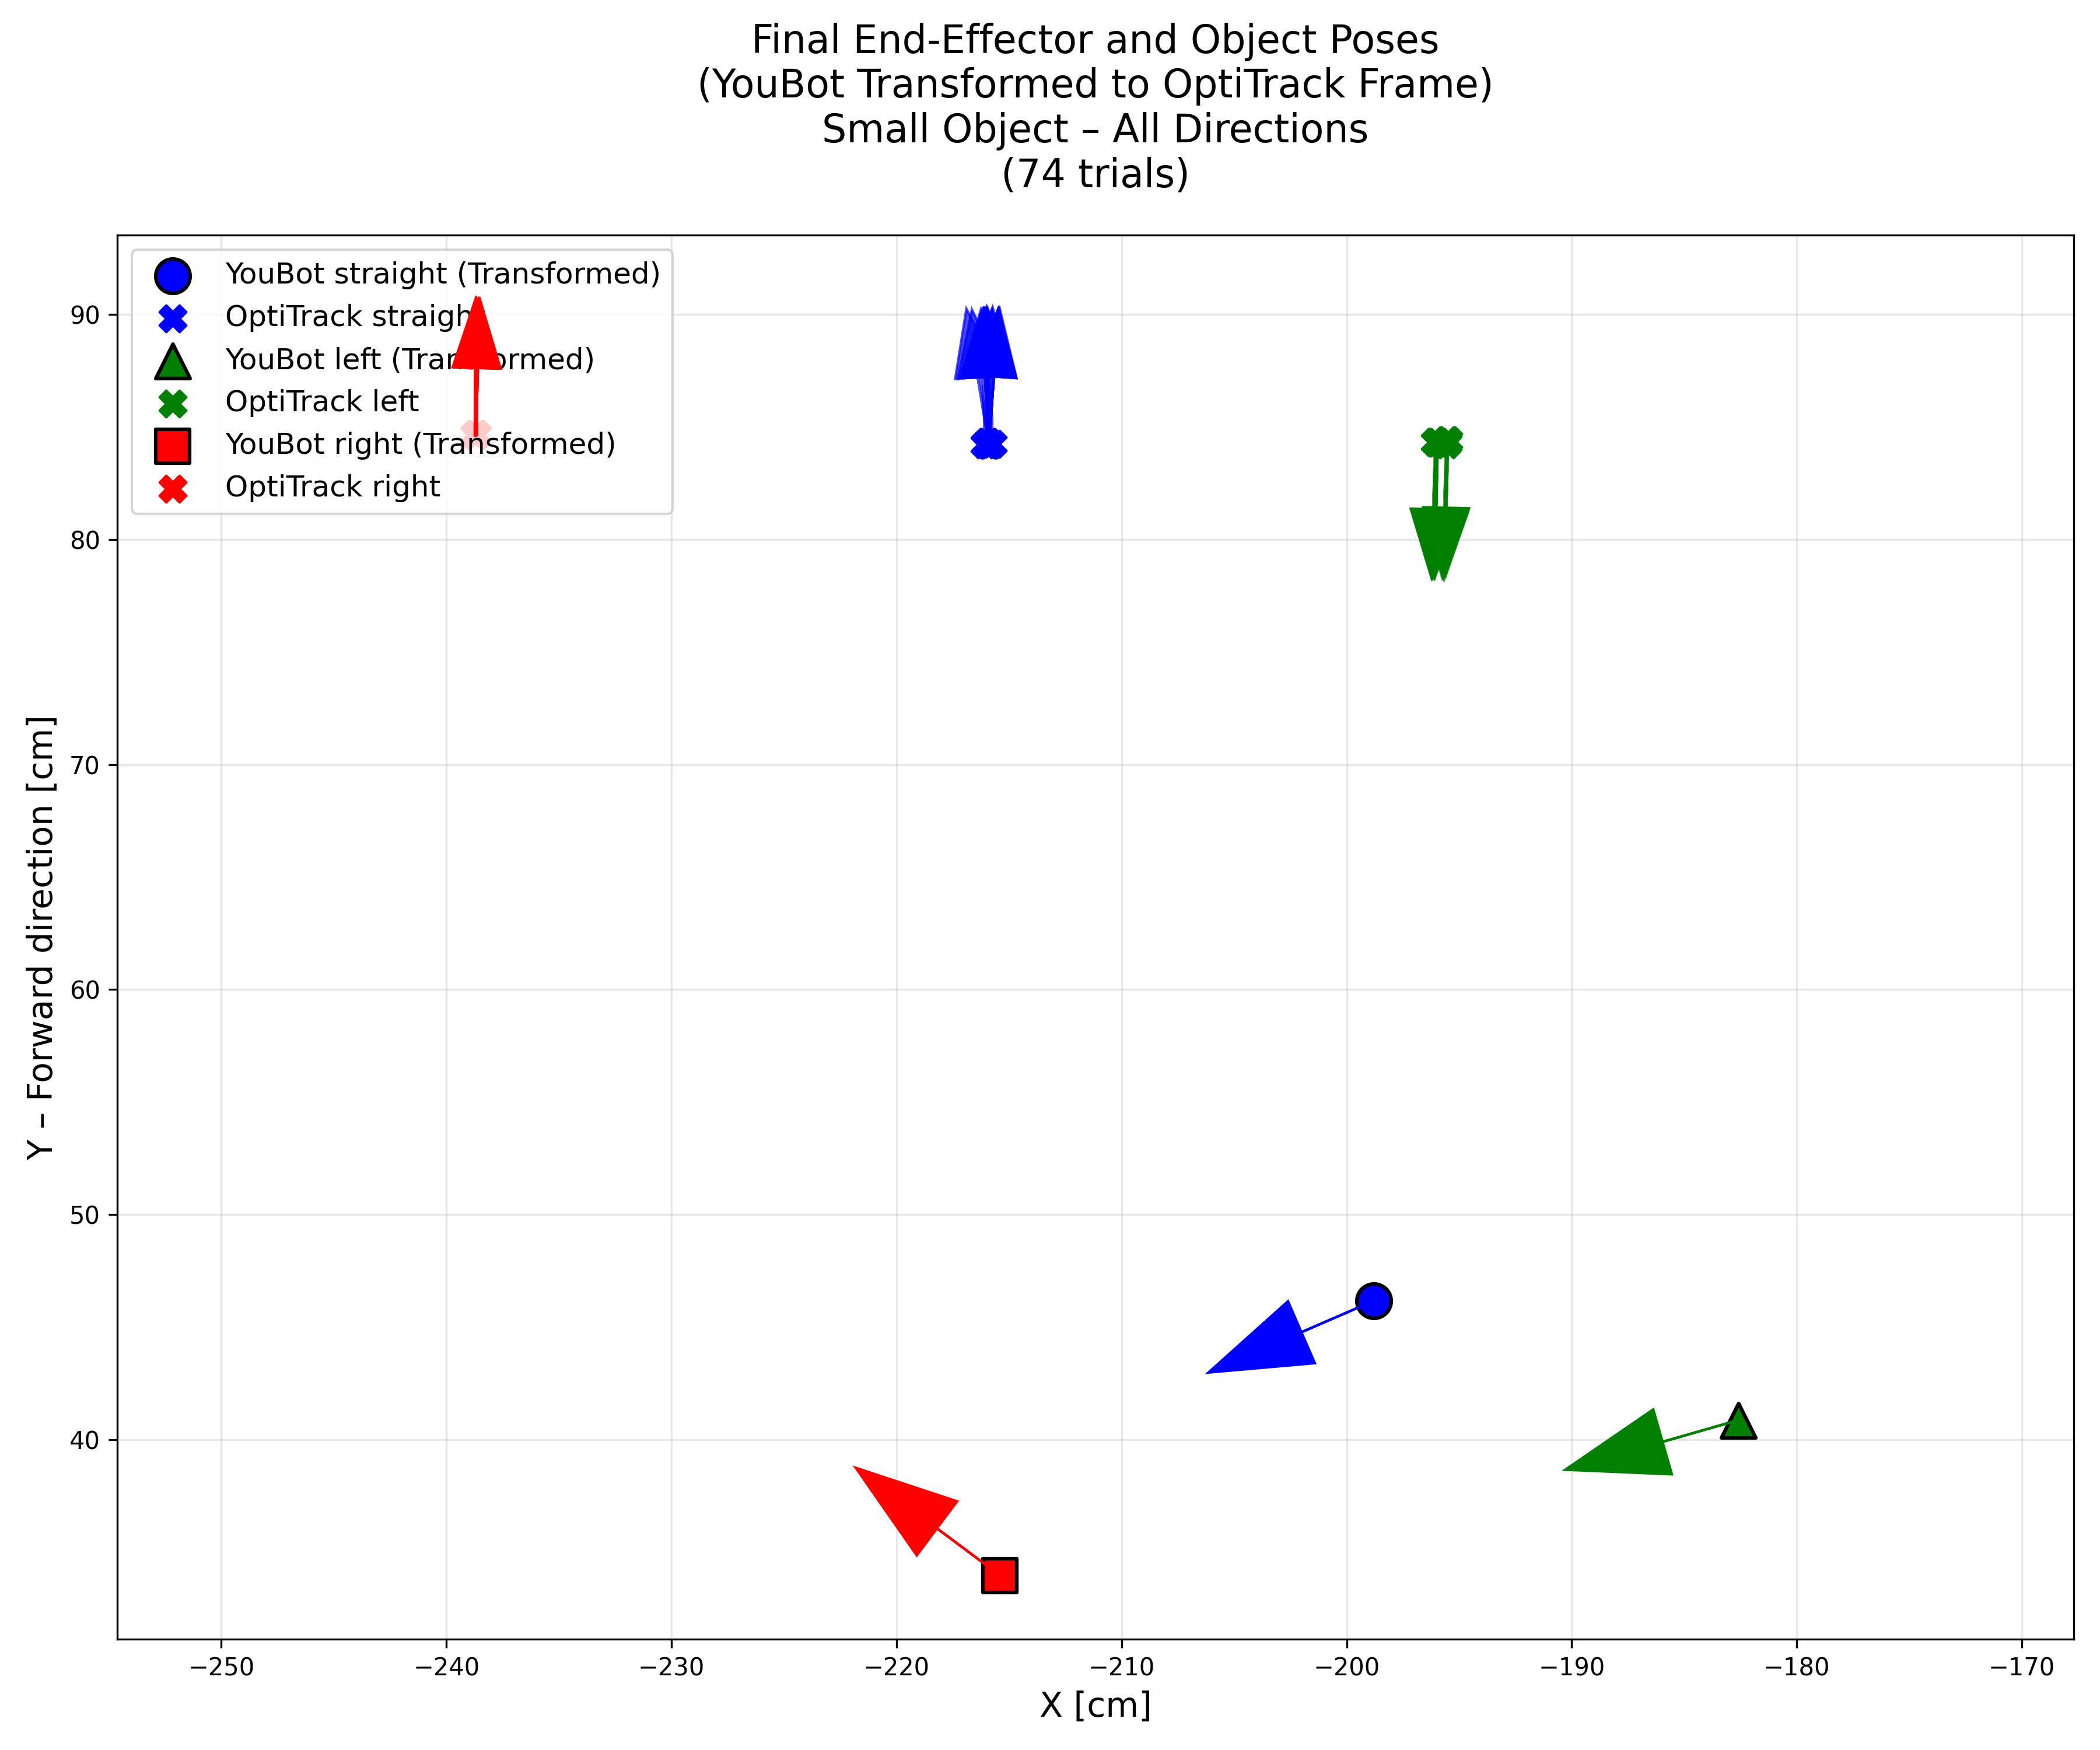
\includegraphics[width=0.4\textwidth]{images/small.png}
    \caption{Final poses for small object across all directions. Circles: YouBot internal, X: OptiTrack external.}
    \label{fig:small}
\end{figure}

\begin{figure}[H]
    \centering
    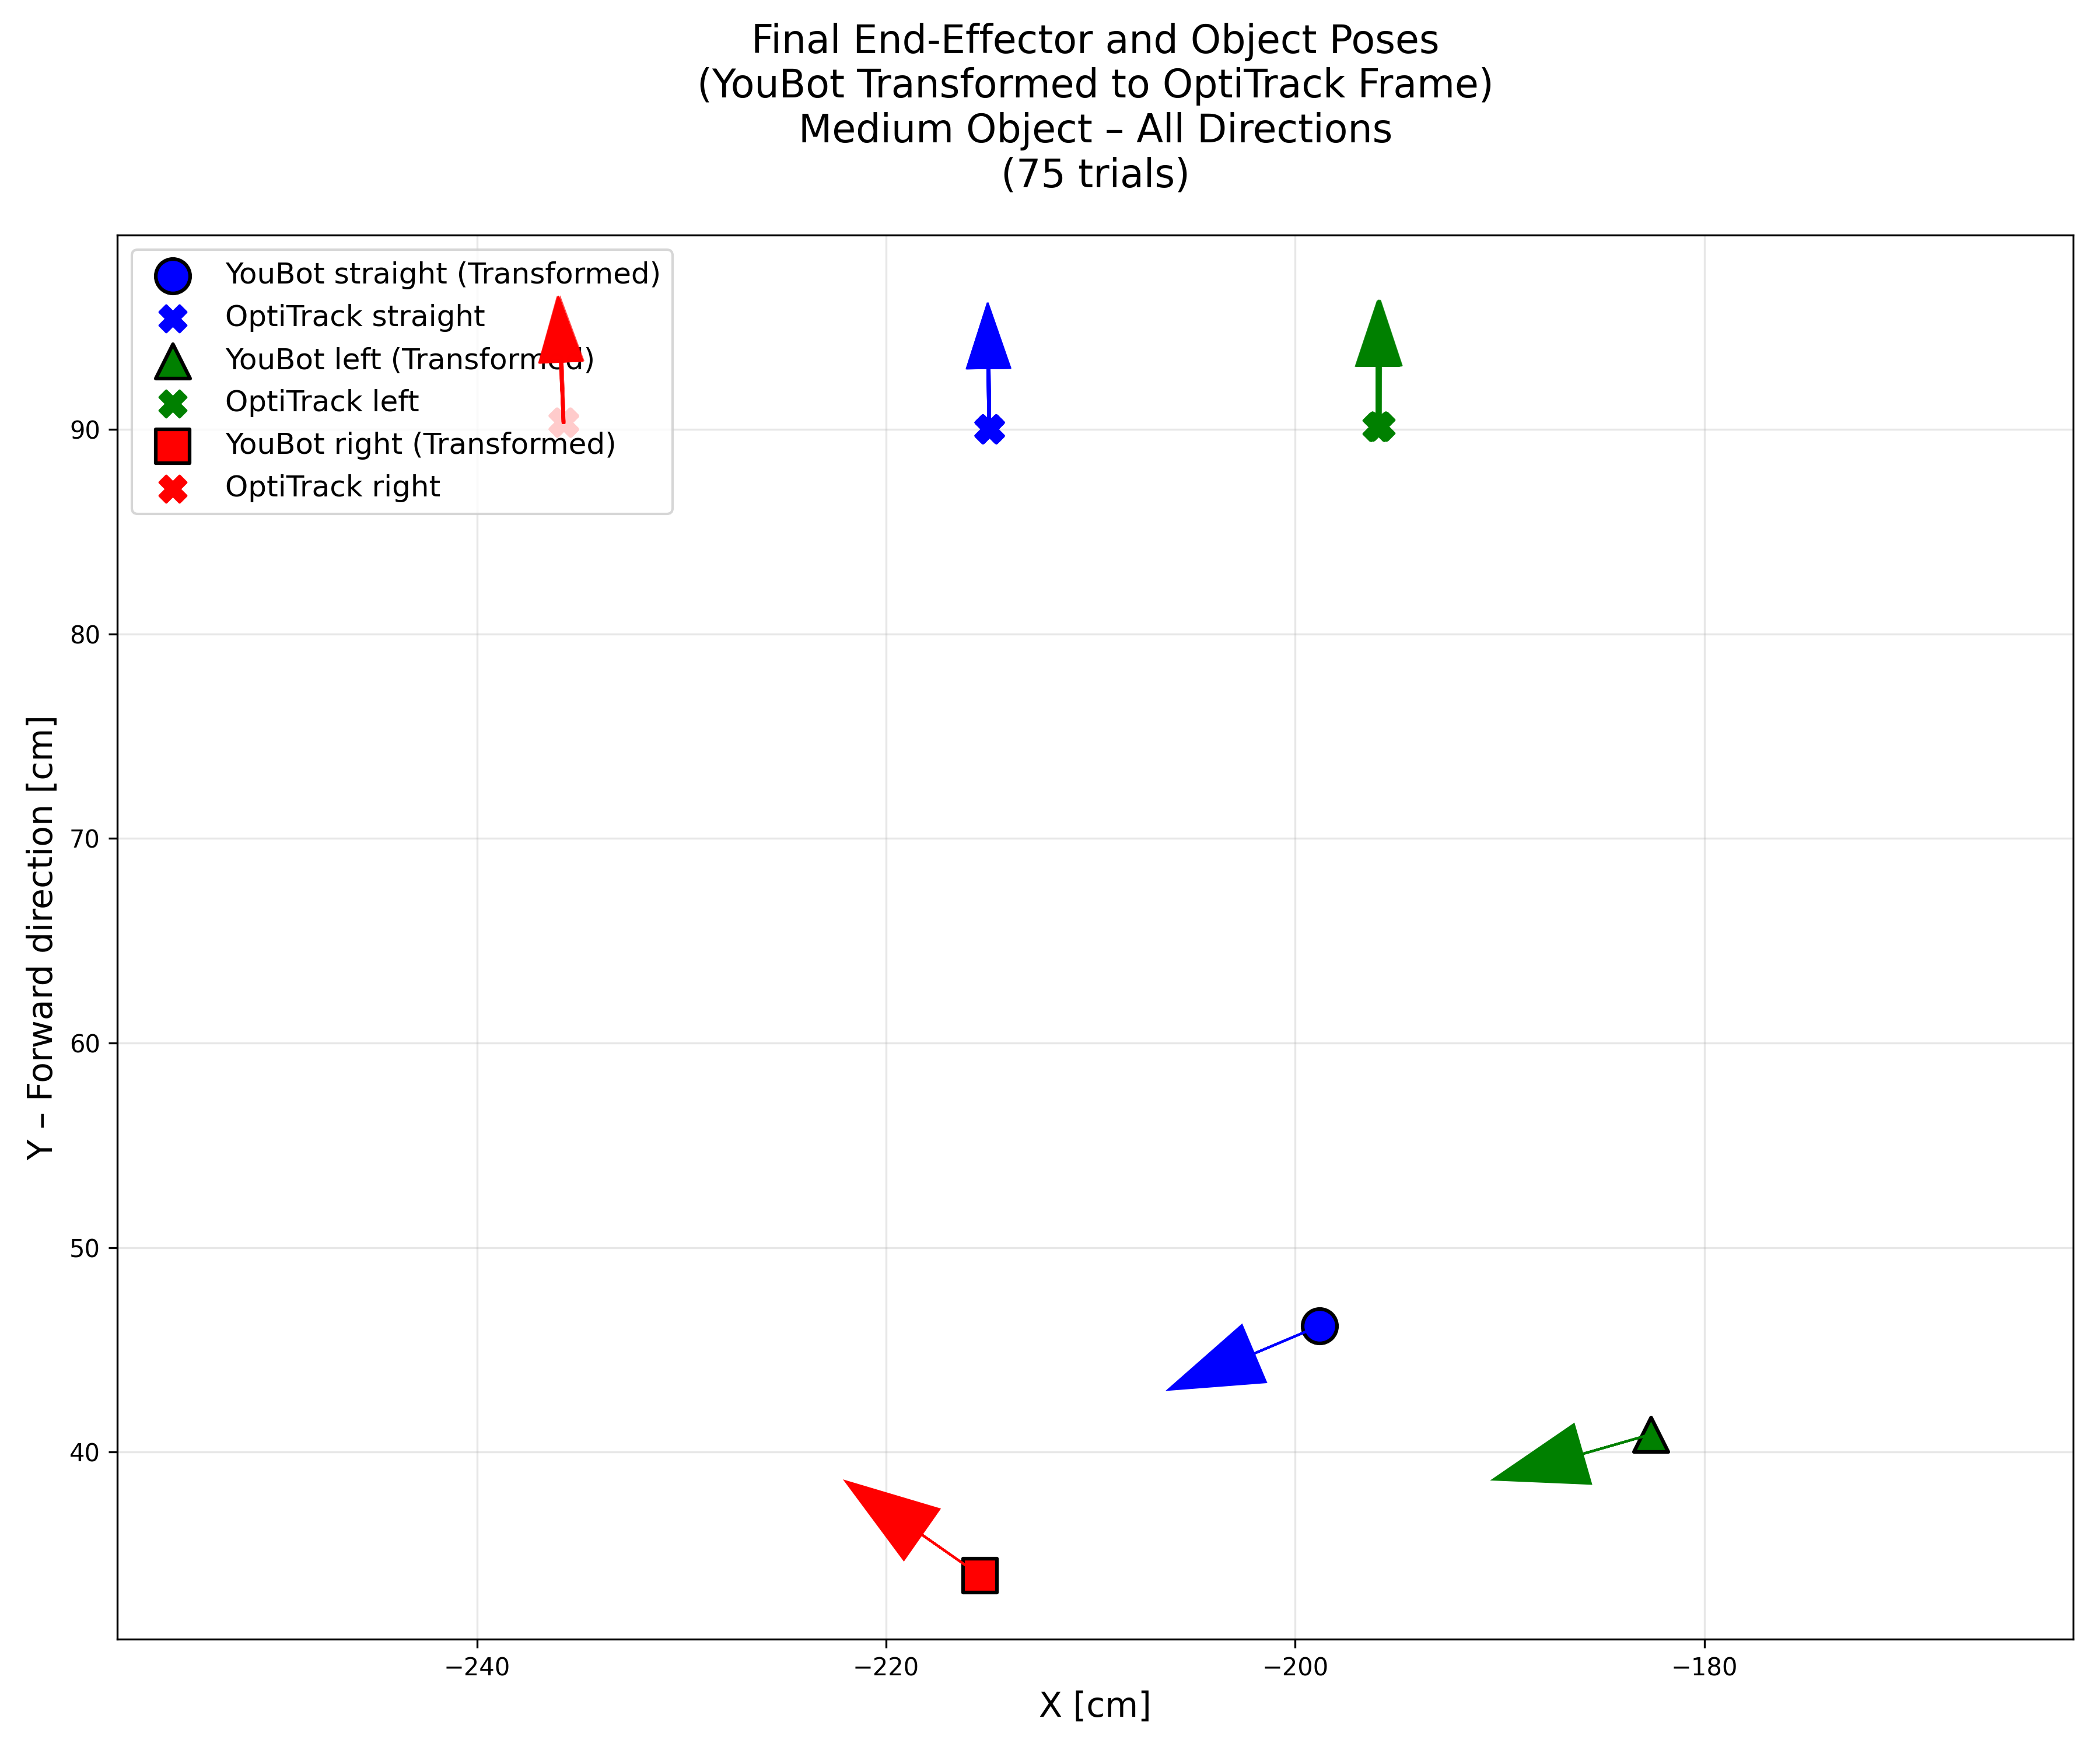
\includegraphics[width=0.4\textwidth]{images/medium.png}
    \caption{Final poses for medium object across all directions.}
    \label{fig:medium}
\end{figure}

\begin{figure}[H]
    \centering
    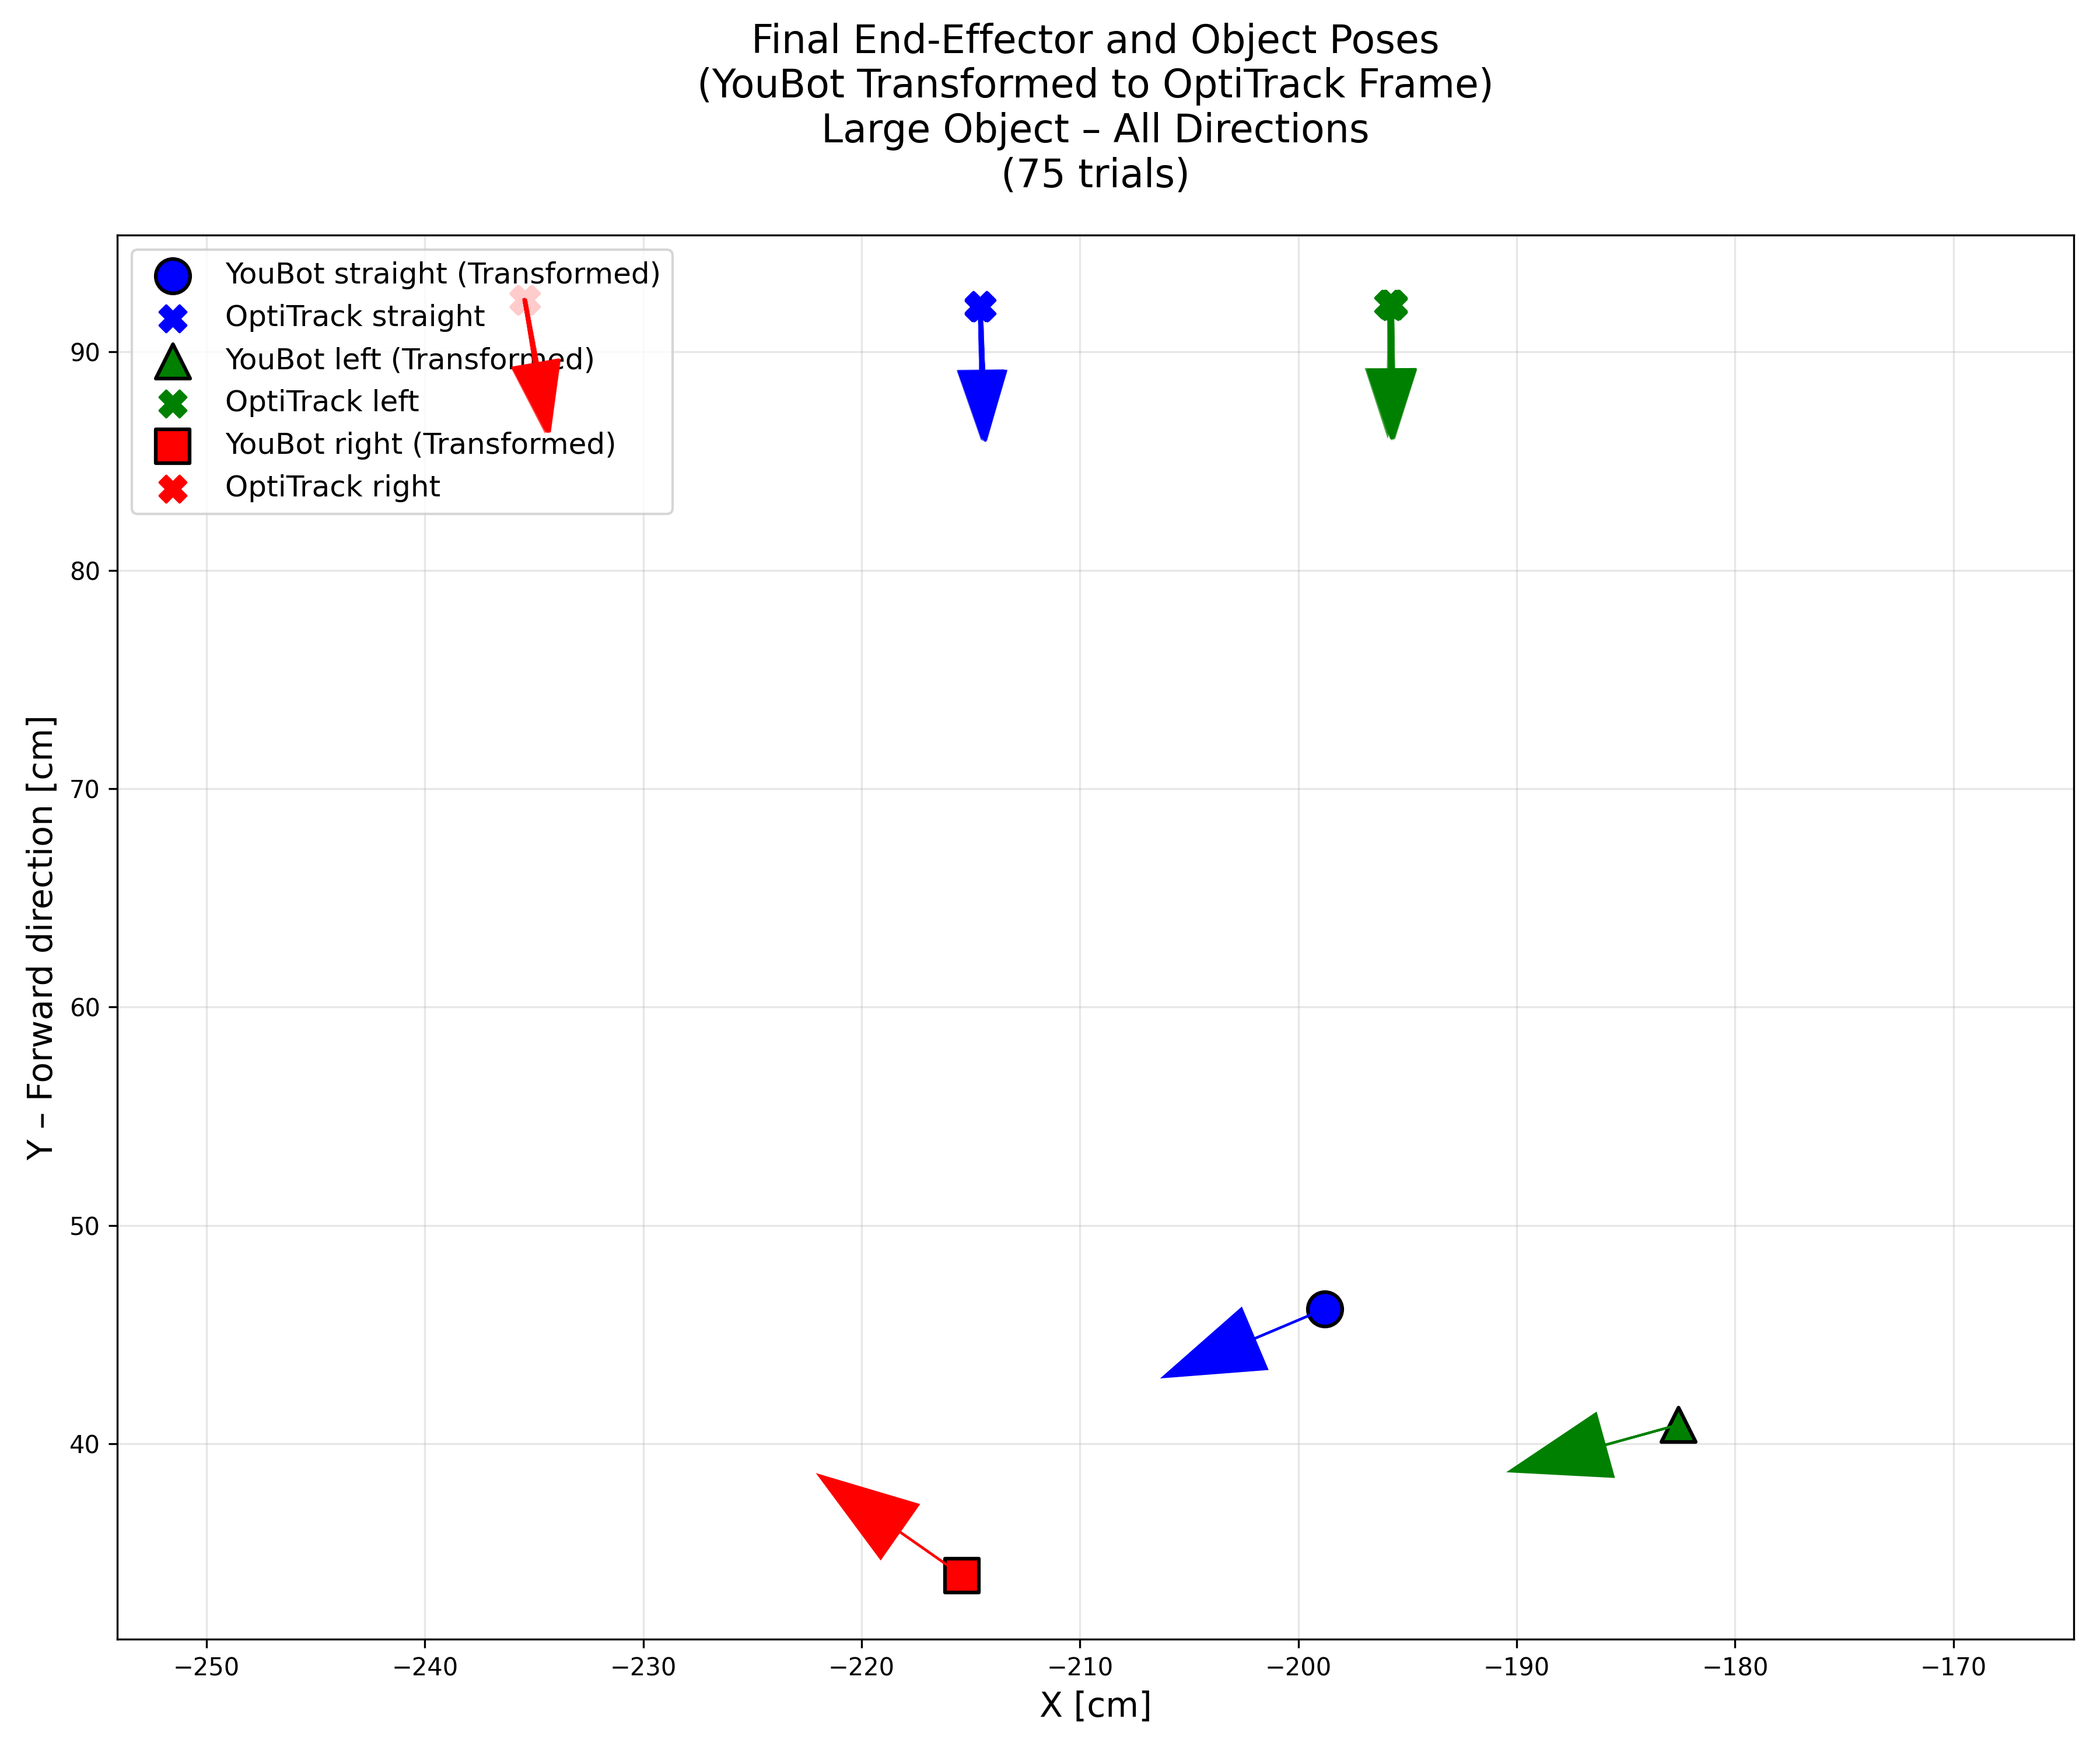
\includegraphics[width=0.4\textwidth]{images/large.png}
    \caption{Final poses for large object across all directions.}
    \label{fig:large}
\end{figure}

The visualizations highlight the distributions per object size, showing how the arm's internal sensing provides consistent target positions while external tracking reveals the actual placement variability. Larger objects show more spread in external measurements, likely due to increased wobbling during placement.



\section{Statistical Analysis}
The analysis estimates accuracy (mean distance between internally sensed end-effector pose and externally tracked object pose) and precision (standard deviation of externally tracked object positions) of the KUKA youBot arm.

\paragraph{Accuracy:}
The mean distances range from approximately 140 cm to 160 cm across different object sizes and directions. This indicates relatively low accuracy, likely due to misalignments between the robot's internal coordinate system and the external tracking system, as well as potential calibration issues. Larger objects show slightly higher mean distances, possibly due to increased wobbling affecting placement.

\paragraph{Precision:}
The standard deviations of object positions are very low, ranging from 0.02 cm to 0.05 cm. This suggests high precision in the arm's repeatability for placing objects. The straight direction generally shows the highest precision, while left and right directions have slightly lower but still excellent repeatability.

\paragraph{Discussion:}
The results highlight a trade-off: while the arm is highly precise in repeating motions, there are significant accuracy issues that may stem from coordinate frame transformations or sensor calibration. Future work could focus on improving alignment between internal and external measurements to enhance overall positioning accuracy.



\section{Combined Analysis Across All Groups}
To provide a comprehensive evaluation, data from all four groups (Group 1, 2, 3, and 4) was combined and analyzed together. This section presents the results of merging datasets from different experimental setups, allowing for a broader assessment of the KUKA youBot arm's performance across varied conditions and implementations.

\subsection{Data Integration}
Data from each group was standardized to common units (cm for positions, radians for orientations) and combined from all available CSV files. The combined dataset includes trials from all groups, sizes, and directions, providing a total of 1200 experimental runs.

The combined preprocessed data is available at:
\href{https://github.com/Nikhil-URG/KUKA-Youbot-RobotArm_Manipulation/blob/main/combined_preprocessed_data.csv}{Combined data}

\subsection{Combined Pose Visualizations}
Visualizations for the combined data show the distribution of final poses across all groups, highlighting both individual group performance and overall trends.

\begin{figure}[H]
    \centering
    
\includegraphics[width=0.4\textwidth]{images/combined_small.png}
    \caption{Combined final poses for small object across all directions and groups.}
    \label{fig:combined_small}
\end{figure}

\begin{figure}[H]
    \centering
    
\includegraphics[width=0.4\textwidth]{images/combined_medium.png}
    \caption{Combined final poses for medium object across all directions and groups.}
    \label{fig:combined_medium}
\end{figure}

\begin{figure}[H]
    \centering
    
\includegraphics[width=0.4\textwidth]{images/combined_large.png}
    \caption{Combined final poses for large object across all directions and groups.}
    \label{fig:combined_large}
\end{figure}

The combined visualizations reveal consistent patterns across groups, with some variations likely due to different experimental setups and environmental conditions.

\subsection{Combined Statistical Analysis}
Statistical analysis on the combined dataset provides insights into overall accuracy and precision across all groups.

\paragraph{Accuracy (Combined):}
The mean distances between internal and external measurements across all groups range from 213.60 cm to 268.62 cm. This combined analysis shows variations across groups and conditions, with Group3 generally showing lower distances than Group1 and Group2.

\paragraph{Precision (Combined):}
The standard deviations of external positions across all groups are 0.01 cm to 0.83 cm, indicating high precision overall, with some variation between groups.

\paragraph{Group-wise Comparison:}
A comparison of accuracy and precision across groups is shown in the following table:

\begin{table}[H]
\centering
\caption{Combined Accuracy and Precision by Group, Size, and Direction}
\label{tab:combined_stats}
\begin{tabular}{|c|c|c|c|c|}
\hline
Group & Size & Direction & Accuracy (cm) & Precision (cm) \\
\hline
Group1 & large & left & 259.53 & 0.20 \\
Group1 & large & right & 268.62 & 0.03 \\
Group1 & large & straight & 259.33 & 0.19 \\
Group1 & medium & left & 258.20 & 0.17 \\
Group1 & medium & right & 267.82 & 0.02 \\
Group1 & medium & straight & 257.71 & 0.13 \\
Group1 & small & left & 255.39 & 0.04 \\
Group1 & small & right & 267.58 & 0.02 \\
Group1 & small & straight & 256.69 & 0.03 \\
Group2 & large & left & 259.52 & 0.02 \\
Group2 & large & right & 268.54 & 0.03 \\
Group2 & large & straight & 259.28 & 0.03 \\
Group2 & medium & left & 257.96 & 0.04 \\
Group2 & medium & right & 267.66 & 0.02 \\
Group2 & medium & straight & 257.83 & 0.02 \\
Group2 & small & left & 257.79 & 0.03 \\
Group2 & small & right & 268.05 & 0.83 \\
Group2 & small & straight & 258.52 & 0.02 \\
Group3 & large & left & 259.10 & 0.04 \\
Group3 & large & right & 268.58 & 0.02 \\
Group3 & large & straight & 258.76 & 0.03 \\
Group3 & medium & left & 258.23 & 0.03 \\
Group3 & medium & right & 267.86 & 0.02 \\
Group3 & medium & straight & 258.14 & 0.01 \\
Group3 & small & left & 255.35 & 0.14 \\
Group3 & small & right & 267.67 & 0.02 \\
Group3 & small & straight & 256.39 & 0.06 \\
Group4 & large & left & 259.72 & 0.05 \\
Group4 & large & right & 269.14 & 0.12 \\
Group4 & large & straight & 258.88 & 0.10 \\
Group4 & medium & left & 258.05 & 0.03 \\
Group4 & medium & right & 267.12 & 0.01 \\
Group4 & medium & straight & 257.57 & 0.02 \\
Group4 & small & left & 255.22 & 0.03 \\
Group4 & small & right & 267.40 & 0.03 \\
Group4 & small & straight & 256.49 & 0.02 \\
\hline
\end{tabular}
\end{table}

% The table above compares performance across groups. Data available at: \href{https://github.com/username/repo/blob/main/combined_stats_table.csv}{combined_stats_table.csv}



\paragraph{Discussion (Combined):}
The combined analysis across all groups demonstrates variations in performance across different experimental setups. Group3 shows the best accuracy, while precision is generally high across all groups. Variations between groups may be attributed to differences in experimental setup, calibration, or environmental factors. This comprehensive evaluation provides a more robust assessment of the youBot arm's capabilities.

\end{document}